\chapter{A full surface: the horizon and the cell}\label{ch:floorbreach}

\section{The statement}

A black hole is the object that holds the most entropy any region of its size and energy can hold: it saturates the
Bekenstein bound~\cite{Bekenstein1981}. Chapter~\ref{ch:blackholes} reads that as IAM's Law at its limit: a surface written to
capacity. The cellular counterpart proposed by the framework is a cell whose pattern is written past what its own copying
can hold, so that the sites that make it that cell drift toward a coin flip. This chapter sets the two side by side, marks
what each step rests on, and separates the structural statement from the numerical one.

\section{The chain of steps}

\begin{enumerate}
\item \textbf{Bekenstein (1973).} A horizon carries an entropy proportional to its area $\mathcal A$~\cite{Bekenstein1973};
      Hawking's temperature fixes the coefficient, $S_{\mathrm{BH}}=\kB\mathcal A/4\lP^2$~\cite{Hawking1975}. \derived{} (established physics)
\item \textbf{Hawking (1975).} The horizon radiates at $T_H=\hbar c^3/8\pi GM\kB$~\cite{Hawking1975}. \derived{} (established physics)
\item \textbf{Landauer (1961).} Each irreversible bit written at a surface at temperature $T$ costs at least $\kB T\ln2$.
      \derived{} (established physics)
\item \textbf{Jacobson (1995).} The Einstein equation follows from $\delta Q=T\,dS$ applied to local Rindler horizons with
      $S\propto\mathcal A$~\cite{Jacobson1995}. \derived{} (established result)
\item \textbf{IAM.} Decoherence-produced classical information contributes to the horizon entropy functional,
      $S=S_{\mathrm{geo}}+S_{\mathrm{info}}$. The framework's single new identification; its cosmological consequences are
      tested in Part~\ref{part:2}. \conjecture
\item \textbf{The cell.} Methylation maintenance is an irreversible binary write at body temperature, charged $\kB\Tb\ln2$ per
      bit (\derived); its fidelity is measured on molecules as a holding energy of $3.41\,\kB T$ per site (\measured); a cell
      whose identity sites move far from its healthy reading has lost the pattern that makes it that cell (\conjecture).
\end{enumerate}

\section{The two surfaces side by side}

\begin{center}\small
\begin{tabular}{@{}p{0.22\textwidth}p{0.34\textwidth}p{0.36\textwidth}@{}}\toprule
 & horizon & cell \\\midrule
encoding surface & Bekenstein--Hawking horizon & chromatin at the identity sites \\
temperature & $T_H$ ($6.2\times10^{-8}$ K for one solar mass) & $\Tb=310.15$ K \\
capacity & $\mathcal A/4\lP^2$ ($1.5\times10^{77}$ bits) & one bit per CpG copy ($\sim2.8\times10^7$) \\
cost per bit & $\kB T_H\ln2=5.9\times10^{-31}$ J & $\kB\Tb\ln2=2.97\times10^{-21}$ J \\
reading & $S$ against $S_{\mathrm{BH}}$ & $A$ = reading over the healthy reading \\
full surface & $S=S_{\mathrm{BH}}$: a horizon forms & every identity site at $\beta=\tfrac12$ \\\bottomrule
\end{tabular}
\end{center}
All entries are \calc. The bit counts differ by $5.4\times10^{69}$ for one solar mass and the temperatures by ten orders of
magnitude. The equation is shared; the parameters are not.

Figure~\ref{fig:p4_surfaces} draws the four rows of the table on one logarithmic axis.

\begin{figure}[htbp]\centering
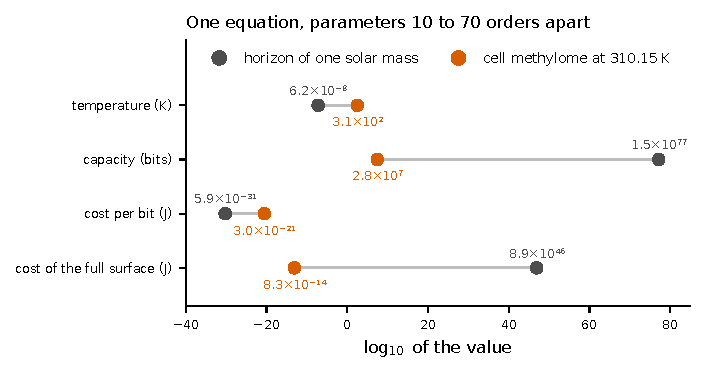
\includegraphics[width=0.72\textwidth]{figures/part6/fig_p4_05_surfaces.pdf}
\caption{The two surfaces of the table above on one axis ($\log_{10}$ of each value). Gray: a horizon of one solar mass; orange: the cell methylome at
310.15~K. The full-surface cost is $T_HS$ for the horizon and $N\kB\Tb\ln2$ for the cell. \calc}
\label{fig:p4_surfaces}
\end{figure}

\section{The full surface of a cell}

A site has a capacity of one bit, reached at $\beta=\tfrac12$. A cell whose identity sites all sit there holds the most
entropy its surface allows, and the gauge then reads its largest possible value, one bit over the healthy reading. For
neutrophils on arrays that is
\begin{equation}
  A_{\max}^{\text{Met-A}}=\frac{1}{0.330263}=3.03,
  \label{eq:Amax}
\end{equation}
and on single molecules, where the copy error itself reaches one half, $A_{\max}^{\text{IAM-A}}=1/(1.149\times0.2043)=4.26$.
\calc{} Both follow from the healthy reference alone; neither is fitted. They are the cell's counterpart of the
Chandrasekhar line on the star gauge of Chapter~\ref{ch:blackholes} (Figure~\ref{fig:stargauge}): the exactly known far end of the gauge.

Figure~\ref{fig:p4_fullsurface} draws both readings from the healthy cell to the full surface.

\begin{figure}[htbp]\centering
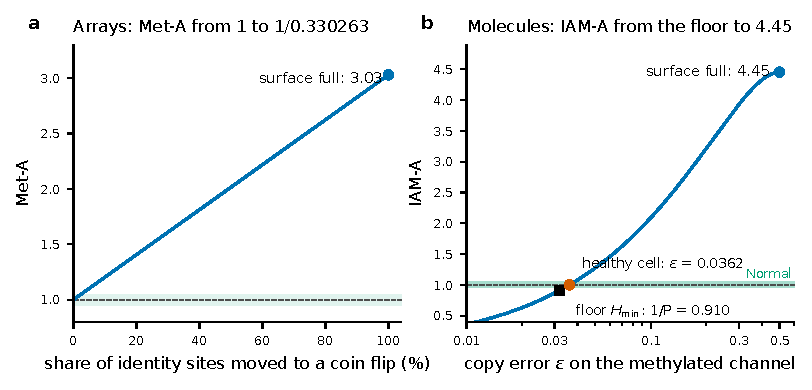
\includegraphics[width=0.95\textwidth]{figures/part6/fig_p4_05_fullsurface.pdf}
\caption{The far end of the gauge, from the healthy reference alone. (a) Met-A when a share of the 6,000 identity sites is moved to $\beta=\tfrac12$:
from 1 to $1/0.330263=3.03$. (b) IAM-A $=H(\varepsilon)/(P\,H(\varepsilon_0))$ against copy error, with $P=1.149$ and
$\varepsilon_0=0.032$: the average healthy cell type ($\Href$) at $1/P=0.870$, the healthy neutrophil at $\varepsilon=0.0384$, the full surface
4.26 at $\varepsilon=\tfrac12$. Normal shaded. \calc}
\label{fig:p4_fullsurface}
\end{figure}

The analog fails in one respect, and we state it plainly. The horizon condition is about a rate of writing
exceeding what a surface can absorb. A reading of the cell's condition as a cell that ``can no longer pay the cost of
remaining itself'' is not supported if cost means energy: methylation maintenance uses of order $10^{-7}$ of the cell's ATP
(Chapter~\ref{ch:landauer}). What the numbers support is a balance of fidelities: a pattern held by a writing process of
finite discrimination against copying errors and active removal. A cell whose balance fails loses the pattern whatever its
energy supply. The full-surface condition for a cell is therefore a failure of maintained fidelity, not of energy.
\conjecture

\section{Direction}

The gauge reads two directions away from $A=1$ (Chapter~\ref{ch:gauge}):
\begin{itemize}
\item \textbf{Above 1}: more error than the healthy cell on its own identity sites. The pattern is becoming uncertain; the
      writing surface is being written faster than it can hold a pattern. This is the direction of the horizon analogy, and the direction tumors have moved: in all ten tumor--normal pairs read so far (six early-onset colorectal, four oral), the tumor's copy error on
      single molecules is above that of the same person's normal tissue; with 5hmC removed, in three of the four oral pairs
      (Chapter~\ref{part4:ch:reach}). \measured{} Where breach and the cancer
      region lie on this side is still to be measured (Chapter~\ref{ch:gauge}).
\item \textbf{Below 1}, toward the floor $\Hmin$ far to the left: less error than the healthy cell. The copies agree more than the healthy
      cell's do. Senescent IMR90 fibroblasts read below Normal on their unmethylated channel (0.685--0.695; Chapter~\ref{ch:gauge}).
      \measured{} What this region means for a cell has not been measured with the current method. \openprob
\end{itemize}
Neither is the same as a cell doing more work. A neutrophil clearing an infection works harder while keeping its identity;
the physics does not predict that activity moves a cell on the gauge (Chapter~\ref{ch:leukocyte}).

\section{What the comparison establishes}

It establishes a \emph{structural} identity: the same cost per bit and the same notion of a full surface at both scales,
with different temperatures and capacities. It does not establish a \emph{numerical} unification, and no shared quantitative
saturation condition across horizons, devices and cells has been shown.
